\section{Training an Insight Anticipator}
We explore two primary training paradigms to optimize \ourmethod{} for insight anticipation: (1) distillation via supervised fine-tuning (SFT), leveraging ground-truth insights and rationalization from target papers, and (2) reinforcement learning (RL) for insight anticipation via similarity optimization. Across all experiments, we adopt \qwenfourb{} as our base model. Next, we will detail the specific formulations of these training methodologies.

\subsection{Ground Truth Insight Distillation via Supervised Fine-Tuning (SFT)}
The objective of our SFT pipeline is to adapt the base language model to synthesize a cohesive, derivative insight given the textual context of two source papers. We investigate two distinct SFT strategies to achieve this. In our standard SFT approach, the model is directly fine-tuned to map the input context (summaries of parent papers), $x$, to the target ground-truth insight, $y^*$ (derived from the target paper). This process optimizes the standard negative log-likelihood loss for autoregressive LMs over the paired examples $(x, y^*)$.

To bridge the logical gap between the source papers and the final insight, we also evaluate an SFT strategy enhanced with chain-of-thought reasoning~\citep{wei2023chainofthoughtpromptingelicitsreasoning}, which we denote as \emph{SFT-think}. In this setup, we introduce an intermediate synthetic rationalization step, $z$. To generate a supervision target, we prompt a high-capacity teacher model (\gemthreepro{}) to generate a detailed chain-of-thought that logically deduces the ground-truth insight conditioned on the parent paper summaries (as detailed in Section~\ref{sec:dataset_construction}). The base model is then trained to sequentially predict the rationale followed by the final insight, utilizing the augmented tuples $(x, z, y^*)$. This approach explicitly encourages the model to internalize the step-by-step inferential process rather than merely memorizing the final output mapping. This follows distillation approaches in reasoning as seen in works such as OpenThoughts~\citep{guha2025openthoughtsdatarecipesreasoning} and s1~\citep{muennighoff2025s1simpletesttimescaling}.

\begin{figure}[t]
    \centering
    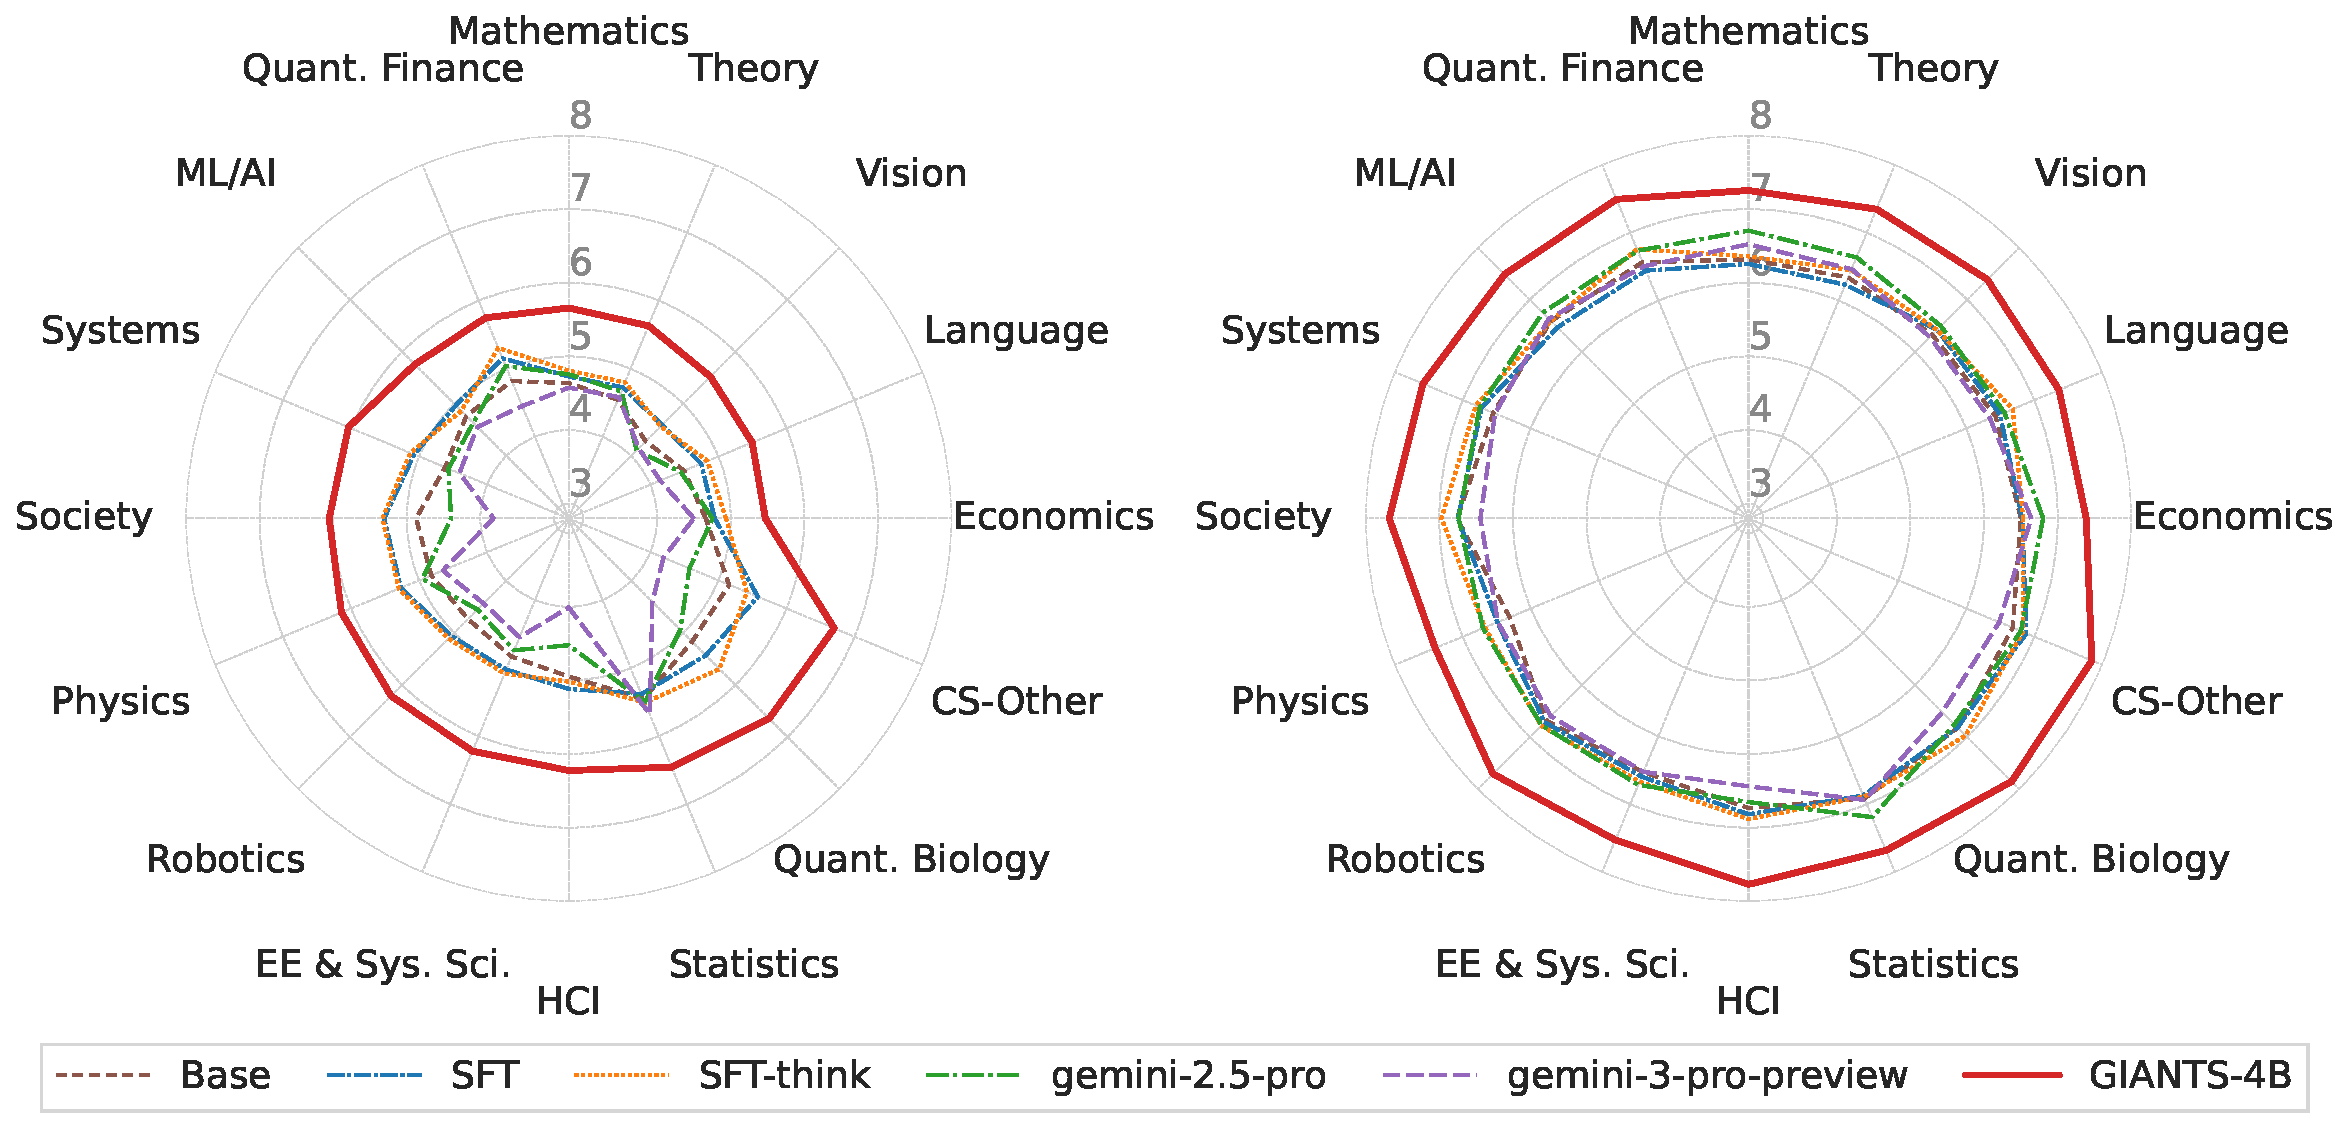
\includegraphics[width=0.9\linewidth]{figs/all_domain_radar_comparison_gemini-3-pro-preview_vs_Qwen3-14B.pdf}
    \vspace{-3mm}
    \caption{\footnotesize \textbf{Insight anticipation for arXiv domains.} \ourmethod{} has a higher similarity score to the target insight, outperforming SFT, SFT-Think, and the base model (\qwenfourb{}) for two different judge models.  The relative ordering of similarity scores for each domain, judged by \gemthreepro{} \textit{(left)} matches the ordering of similarity scores judged by \qwenfourteenb{} \textit{(right)}.}
    \label{fig:all_domain_radar_comparison_gemini-3-pro-preview_vs_Qwen3-14B}
\end{figure}

\begin{figure}[t]
    \centering
    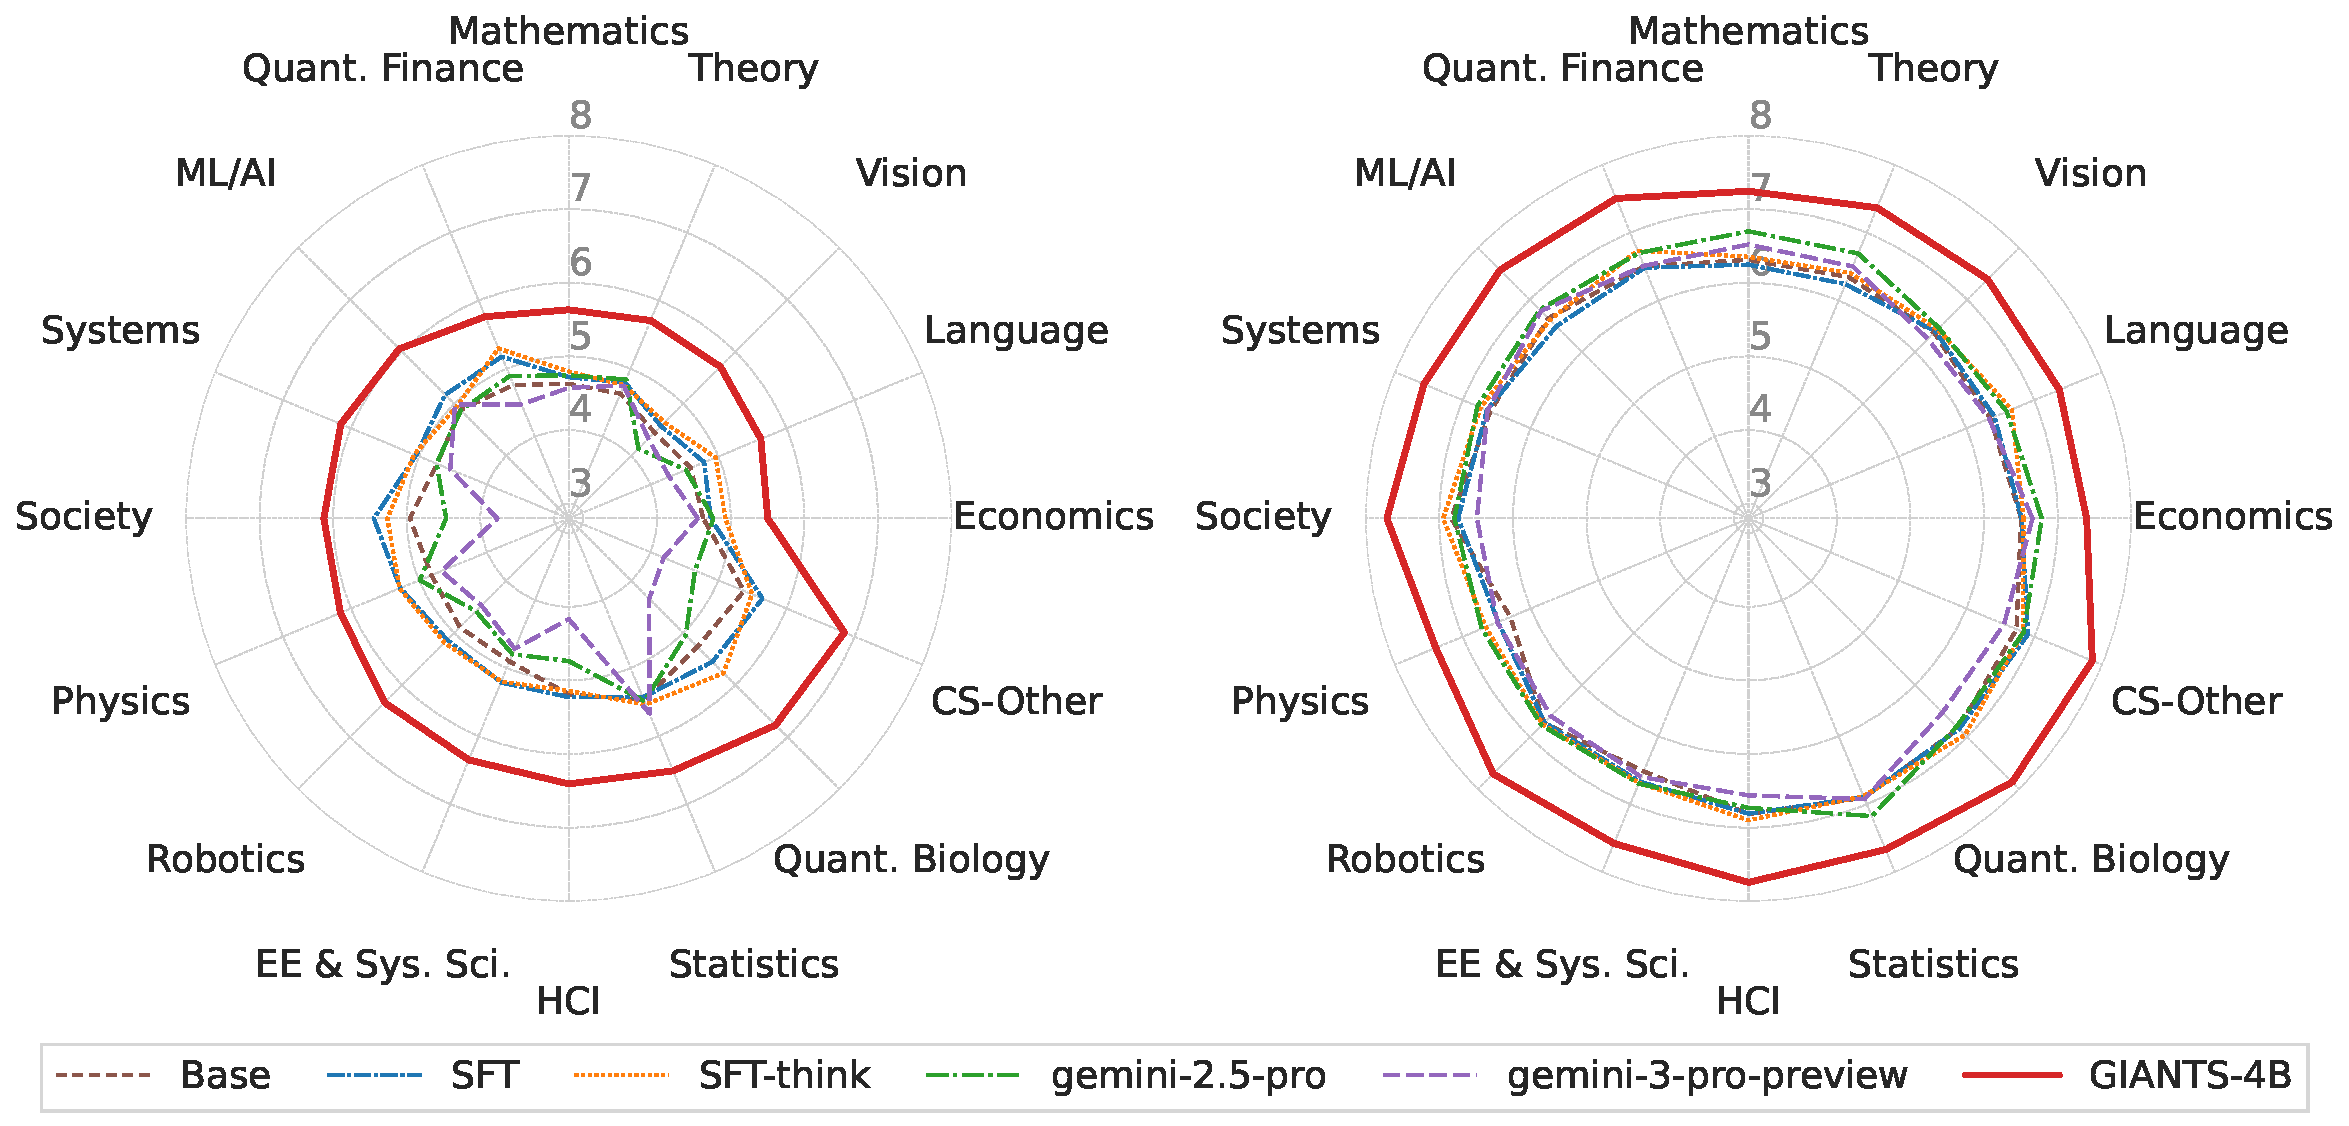
\includegraphics[width=0.9\linewidth]{figs/all_domain_radar_comparison_gemini-3-pro-preview_vs_Qwen3-14B_unseen_parents.pdf}
    \vspace{-3mm}
    \caption{\footnotesize \textbf{Similarity scores on \emph{Test-unseen-parents}}. This is the subset of \ourbenchmark{} test set with only unseen parent papers, where \ourmethod{} outperforms the base model and SFT both when judged by \gemthreepro{} \textit{(left)} and \qwenfourteenb{} \textit{(right)}.}
    \label{fig:all_domain_radar_comparison_gemini-3-pro-preview_vs_Qwen3-14B_unseen_parents}
    \vspace{-3mm}
\end{figure}

% (1) directly finetuning on $(x, y^*)$, and (2) finetuning on $(x, z, y^*)$ where the model generates chain-of-thought reasoning $z$ before the insight statement $y^*$. In the training data, $z$ is the generated by \qwenfourteenb{} when rewriting the insight (see Section~\ref{sec:dataset_construction}).

% The LM as Judge thing seems a bit weaker -> Changed to Insight Similarity
\subsection{Reinforcement Learning for Insight Anticipation via Similarity Optimization}
So far, we have explored distilling insights via supervised fine-tuning (SFT). However, in complex tasks such as scientific discovery, the target paper's insights can be difficult to clone directly. This difficulty often arises when the target insight has low likelihood under the policy, or when the model lacks the capacity to adequately capture the distribution of the parent insight. Can we instead consider an alternative approach that relies on reinforcement learning to recover the performance of the target paper's insights?

To address this, we employ an alternative approach: using the target paper's insights $y^{*}$ to define a proxy reward via a semantic similarity metric. Formally, given an insight from the target paper $y^{*}$, we define the proxy reward for a predicted insight $\hat{y}$ as: 
\begin{align}
    r_{\text{sim}}(\hat{y}) = \textit{similarity}(\hat{y}, y^{*})
\end{align}
where $\textit{similarity}$ measures the semantic equivalence between the generated insight and target insights measured using an LM-as-a-Judge~\citep{gu2025surveyllmasajudge}, matching the evaluation criterion in Section~\ref{sec:dataset_construction}. Furthermore, for further robustness and reducing order bias, we supply the LM with insights twice ($\hat{y}$ first, and $y^{*}$ first), taking the average over the individual similarity scores to compute the proxy reward. 
This proxy reward is then optimized via RL to recover the behavior of the ground-truth insight of the child paper conditioned on the two prespecified parent papers.

More concretely, we train \ourmethod{} using Group Relative Policy Optimization (GRPO) \citep{shao2024deepseekmath}, utilizing an LM as a proxy reward function. Specifically, for each input context $x$, we sample a group of $G=8$ candidate insights from the active policy. An LM judge evaluates these candidates and assigns scalar rewards based on a predefined similarity score metric (illustrated in Figure~\ref{fig:giants_fig1}, bottom). GRPO is well-suited for this setup because it optimizes the policy relative to the sampled group, thereby removing the need to train and maintain a separate, memory-intensive value function model.

Crucially, to mitigate the risk of reward hacking and ensure a rigorous evaluation, we enforce a strict separation between the training and testing judges. We deploy \gemtwoflash{} as the active reward model during GRPO training, while reserving the independent \gemthreepro{} model exclusively for the final evaluation phase. This decoupling guarantees a more objective, unbiased assessment of the model's true generalization capabilities. We additionally evaluate with other LM judges (e.g., \qwenfourteenb{}) to showcase robustness across model families.
% \footnote{\href{https://huggingface.co/Qwen/Qwen3-14B}{https://huggingface.co/Qwen/Qwen3-14B}}

\begin{AIbox}{Takeaways of Training an Insight Anticipator}
We optimize our insight anticipator using reinforcement learning to maximize semantic similarity to target insights. We strictly separate the LLM judges used for training and final evaluation.
\end{AIbox}


% Old Text
\iffalse

 We explore two training approaches: (1) Supervised fine-tuning on ground-truth insights, and (2) Reinforcement learning with an LLM as a judge. For all experiments we use \qwenfourb{} as the model being trained.


A base LM is fine-tuned to generate the downstream insight given two parent papers using standard supervised objectives. We compare two SFT approaches: \begin{itemize} \vspace{-10pt} \item \textbf{SFT}: We finetune the model on $(x, y^*)$. \vspace{-6pt} \item \textbf{SFT-think}: We generate synthetic chain-of-thought reasoning $z$ that leads to the ground-truth insight by prompting \gemthreepro{} (see Section~\ref{sec:dataset_construction}). Then, we conduct SFT on these synthetic thoughts with the ground-truth insights (i.e., $(x, z, y^*)$). \end{itemize}

We train \ourmethod{} using Group Relative Policy Optimization (GRPO; \citet{shao2024deepseekmath}) with rewards provided by an LM judge. Note that we use \gemtwoflash{} as the LM judge in training, different from the judge \gemtwopro{} in testing, to ensure a more reliable and unbiased evaluation. For each context, we sample $G=8$ candidate responses and compute rewards based on the similarity score evaluated by the LM judge (Figure~\ref{fig:giants_fig1}, right).
 
\fi

% \subsection{Frontier Model Baselines}
% We evaluate large frontier language models using zero-shot prompting as a reference baseline.

% TODO: try other model families


% \paragraph{LM-Based Similarity Judgment.}

% Our primary evaluation signal is based on a language model acting as a judge. For each generated insight, the judge assigns a similarity-based score comparing the model-generated insight to the ground-truth insight of the downstream paper.

% This similarity score is used both: (1) As a reward signal during reinforcement learning fine-tuning, and (2) As the main quantitative metric for comparing model variants at evaluation time.

% This approach enables scalable evaluation over a large corpus of papers, but raises the question of how well the LM-based judgments align with human evaluations.



% \subsection{Implications for Evaluation}

% Taken together, these results suggest that LM-based judgment provides a noisy but informative evaluation signal. While absolute score calibration remains imperfect, the strong correlation with human consensus supports its use for:
% \begin{itemize}
%     \item Model comparison
%     \item Reinforcement learning optimization
%     \item Large-scale evaluation where human annotation is infeasible
% \end{itemize}

% We therefore treat LM judgment as an approximate but practically useful proxy for human evaluation, and report human validation results to contextualize its limitations.




